%\documentclass{report}
%%
%\usepackage[english]{babel}
\usepackage{illcmolthesis}
\usepackage{microtype}
\usepackage{amsmath,amssymb}
\usepackage{amsthm}
\usepackage[round, authoryear]{natbib}
\usepackage[all]{xy}
\usepackage{array}
\usepackage{graphicx}
\usepackage{framed}
\usepackage{enumerate}
\usepackage{qtree}
\usepackage{mdframed}
\usepackage{tikz}
\usepackage{multirow}
\usepackage{pgfplots}
\pgfplotsset{compat = newest}
\usepackage{tikz-dependency}
\usepackage{xfrac}
\usepackage{algorithmic}
\usepackage{algorithm}
\usepackage{float}
\usepackage[OT2,T1]{fontenc}
\usepackage{hyperref}
\newcommand\textcyr[1]{{\fontencoding{OT2}\fontfamily{wncyr}\selectfont #1}}
\newcommand{\myparagraph}[1]{\paragraph{#1}\mbox{}\\}
\bibliographystyle{plainnat}
\renewcommand\topfraction{0.85}
\renewcommand\bottomfraction{0.85}
\renewcommand\textfraction{0.1}
\renewcommand\floatpagefraction{0.85}

%Define theorem style for definition and metric
\newtheoremstyle{break}  % follow `plain` defaults but change HEADSPACE.
  {\topsep}   % ABOVESPACE
  {15pt}   % BELOWSPACE
  {\itshape}  % BODYFONT
  {0pt}       % INDENT (empty value is the same as 0pt)
  {\bfseries} % HEADFONT
  {.}         % HEADPUNCT
  {\newline}  % HEADSPACE. `plain` default: {5pt plus 1pt minus 1pt}
  {}          % CUSTOM-HEAD-SPEC

\theoremstyle{break}
\newtheorem{metric}{Metric}
\newtheorem{notion}{Notion}
\newtheorem{definition}{Definition}
\def\citepos#1{\citeauthor{#1}'s (\citeyear{#1})}

%Define new float environment for tables that is boxed
\floatstyle{boxed}
\newfloat{tab}{tbp}{lop}
\floatname{tab}{Table}
\newcommand{\G}{\mathcal{G}}
\newcommand{\Hg}{\mathcal{H}}
\newcommand{\N}{\mathcal{N}}
\newcommand{\C}{\mathcal{C}}
\newcommand{\Pp}{\mathcal{P}}

%\begin{document}
\chapter{Discussion and Future Work}

In this thesis, we have tried to make a small step to a better understanding of compositional translation, and its feasibility for translation between two natural languages, by empirically analysing the patterns that can be found in translation data. After we motivated the need for such a better understanding and discussed related work (Chapter 2 and 3), we have laid out the framework that we used (Chapter 4), and presented and discussed the results (Chapter 5). In this chapter, we will discuss two things.

Firstly, we will look back at the work in this thesis, and discuss how well the results satisfy our expectations and how they can be interpreted from a wider perspective (Section \ref{sec:discussion}). Secondly, we will propose a possible extension of this work, that can hopefully be the start of a new research project. As all previous chapters in this thesis, this chapter - and therefore this thesis - will end with a brief summary.

\section{Discussion}
\label{sec:discussion}

In the introduction of this thesis, we formulated 3 research questions:\begin{enumerate}
\item Are the compositional structures suggested by dependency parses universal for language?
\item What are the reasons dependency structures deviate during translation?
\item Can dependency parses be used to construct a bilingual compositional grammar?
\end{enumerate}

Before we discuss the answers that we have found to these questions, we would like to take a step back, and recall the reasons that we asked exactly these questions.

\subsection{Compositional Translation from an Empirical Perspective}

In the first chapters of this thesis, we have argued for an empirical approach to compositionality. Theoretically, it seems almost impossible to establish how compositional translation is, because compositionality - although often described by a seemingly simple definition - is a very flexible concept. Empirically, however, we can study the structures that exist in translation data, quantify how reasonable it is that they are generated by a compositional system, and gain information about what this system looks like. If we can find a method to consistently pick one of the compositional structures that is supported by the data for every sentence, this is, with the parsing techniques we dispose of today, likely to be extendible to unknown sentences, and therefore gives a solid grounding to compositional translation as a strategy. 

\subsection{Finding Consistency}

Of course, finding consistency in a corpus of trees is far from trivial if no external information is used at all, which can be easily understood when looking at the following three trees:

\begin{figure}[!ht]
\centering
\begin{tabular}{m{3.2cm}m{3.2cm}m{3.2cm}}
\Tree [ [. Mary ] [. [. loves ] [. John ] ] ] & \Tree [ [. John ] [. [. loves ] [. Mary ] ] ] & \Tree [ [. Eat ] [ [. the ] [. pasta ] ] ]
\end{tabular}
\end{figure}

Intuitively, the first two sentences are very similar - they express similar meanings with a similar form - while the third sentence is somewhat different. From only the trees, this observation cannot be easily captured, as the only thing they differ in are the leafnodes. Without knowledge of the world to tell us that `John' and `Mary' are in some sense comparable to each other, but not really to pasta, and that `loves' takes two arguments, it is nigh impossible for a computer to detect the systematicity in these sentences. That is not to say, that it is entirely impossible \citep[see e.g.,][for an almost completely unsupervised account of structure learning]{bod2006unsupervised}, but to make this computationally feasible many simplifying assumptions are necessary.

In this thesis, we therefore chose to look at a subproblem: the incorporation of monolingual information about the predicate argument structures of the source sentences. Given the elaborate monlingual knowledge about language already available in the scientific world, it seems sensible not to start from scratch, but to build on previous research. Although there are several studies that investigate the correspondence between translation structures and constituency structures, investigations about the usefulness of dependency grammars for MT seem to be underrepresented in literature. In this thesis, we provided such an investigation, focusing on the previously mentioned questions.

\subsection{Summary of Results}

As the results were elaborately discussed in the previous chapter, we will now suffice with a short summary, and focus on the conclusions that can be drawn from them.

Initially, we looked at the suitability of dependency parses as a bilingual system on themselves. We found that plain dependency relations as they are, are not sufficient to consistently select compositional translation trees for a corpus. Although dependency parses have a strong semantic motivation, the structures they prescribe are rarely entirely preserved during translation, and for none of the language pairs considered the overall consistency according to the dependency parses was much higher than 50\%. 

A large part of this inconsistency should be attributed to the fact that dependency parses are generally quite flat, which is undesirable for a bilingual grammar and conflicts with the precondition we imposed on the compositional translation trees we considered (maximal recursivity). When deeper versions of dependency parses were considered, the consistency of the selected trees according to the dependency parses was at least 50 percentage point higher for all datasets.

However, to learn a bilingual grammar that can successfully predict the compositional structures of new sentences, even an 80\% consistency is still quite low. With a manual analysis, we investigated whether the lower scores were assigned to sentences that are intuitively not compositionally translated, or were caused by other reasons. The results of this analysis were hopeful. We found that errors in the data were a prevalent reason for low scores, as well as small phrasal translations that seemed to know a certain systematicity (e.g., the translation of prepositions was often problematic). Although the investigated corpus was small (2 times 100 sentences), these results make us optimistic for the future of compositional translation.

\subsection{Conclusion}

With the results summarised in the previous susbsection, we have satisfactory answered our first two questions, but we have not found a conclusive answer to the third one. Although our results indicate that there is some systematicity to the issues that are troublesome for finding consistency through dependency parses, we have not tested whether dealing with some of these issues could significantly improve the result. Although we believe that such adaptations can be effective, we have serious doubts about the scalability and robustness of such an approach. Rather, we think that a statistical learning approach that uses information from dependency parses (rather than strictly following it), would be more effective to learn such adaptations, and would be more robust to errors. In the remainder of this chapter, we propose an approach to efficiently \textit{learn} a grammar using HATs and dependency grammars. Although an implemented version of the algorithms is available, we will leave the execution and evaluation of the resulting system for future work.


\section{Learning a Compositional Grammar using Dependency Information}
\label{sec:future}

In this section, we will describe the algorithms and techniques that can be used to learn a bilingual grammar from dependency parses using the Expectation Maximization algorithm \citep{dempster1977maximum}. The focus lies on learning the source side of this bilingual grammar, the fact that alignment constraints are taken into account in designing this grammar ensures that the resulting source grammar indeed has a counterpart in the target language.

There are two main obstacles for learning a bilingual grammar from a translation corpus:\begin{enumerate}
\item We cannot compare the structures for different sentences, and therefore we cannot detect similarities or differences.
\item For every sentence, we have many structures, and we do not know how to interpret these structures. That is, a compositional translation of a sentence is described by \textit{one} structure, and we do not know which of these structures should be preferred over other structures.
\end{enumerate}

In this section, we will propose methods to encounter both these issues.

\subsection{Comparing structures}

Machines can only detect patterns in a set of structures if they have information that allows them to compare these. As is quite usual, we will provide this information by labelling the parts (nodes) of the structures. To some of the readers this may seem obvious, but we will provide a small example to illustrate it, revisiting the the following three trees:

\begin{figure}[!ht]
\centering
\begin{tabular}{m{3.2cm}m{3.2cm}m{3.2cm}}
\Tree [ [. Mary ] [. [. loves ] [. John ] ] ] & \Tree [ [. John ] [. [. loves ] [. Mary ] ] ] & \Tree [ [. Eat ] [ [. the ] [. pasta ] ] ]
\end{tabular}
\end{figure}

\noindent Intuitively, the first two sentences are very similar - they expresses similar meanings with a similar form - while the third is somewhat different. This observation cannot be easily captured by a machine, as it lacks the world knowledge to make this inference. However, if it had seen the following structures:

\begin{figure}[!ht]
\centering
\begin{tabular}{m{3.5cm}m{3.5cm}m{3.5cm}}
\Tree [.sentence [.subj Mary ] [.tverb+dobj [.tverb loves ] [.dobj John ] ] ] & \Tree [.sentence [.subj John ] [.tverb+dobj [.tverb loves ] [.dobj Mary ] ] ] & \Tree [.sentence [.tverb Eat ] [ [.det the ] [.dobj pasta ] ] ]
\end{tabular}
\end{figure}

\noindent A machine could have used the node labels to figured out that the first two trees are structurally more similar to each other than to the third tree.

However, consistently providing labels for all nodes of all trees in a corpus is not a trivial task, as monolingual analyses of sentences typically only provide labels for a subset of all spans. We will propose a method to label all spans of a sentence, based on dependency parses, such that the labels are consistent over the corpus.

\subsubsection{Basic Labels}

As dependency parses assign labels to relations between words, they do not directly provide labels for spans. As earlier in this thesis, we will circumvent this issue by interpreting a relation X between A and B as a relation between A and the phrase headed by B. This last phrase will be assigned label X. If word B is not assigned a label by following this procedure, it will be labelled `B-head'. Figure \ref{fig:basic_labels} provides an example.

\begin{figure}
\centering
\begin{tabular}{cc}
\footnotesize{\begin{dependency}[theme=simple]%[hide label]
\begin{deptext}[column sep=.5cm, row sep=.1ex]
My \& dog \& also \& likes \& eating \& sausage \\
\end{deptext}
\deproot{4}{}
\depedge{2}{1}{poss}
\depedge{4}{2}{nsubj}
\depedge{4}{3}{xvmod}
\depedge{4}{5}{xcomp}
\depedge{5}{6}{dobj}
\end{dependency}}\\\\ 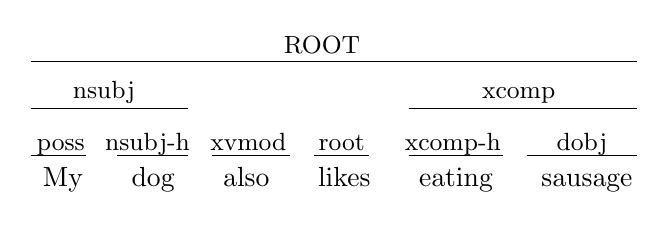
\begin{tikzpicture}
\node at (4,0) {My \hskip 5mm dog \hskip 5mm  also \hskip 5mm  likes \hskip 5mm  eating \hskip 5mm  sausage};
\draw (0.1, 0.3) -- (0.8,0.3);
\draw (1.2, 0.3) -- (2.1,0.3);
\draw (0.1, 0.9) -- (2.1, 0.9);
\draw (2.4, 0.3) -- (3.4,0.3);
\draw (3.7, 0.3) -- (4.4,0.3);
\draw (4.9,0.3) -- (6.1,0.3);
\draw (6.4,0.3) -- (7.8,0.3);
\draw (4.9,0.9) -- (7.8,0.9);
\draw (0.1,1.5) -- (7.8, 1.5);
\draw (3.7,1.1) node [font=\small] {nsubj \hskip 43mm xcomp};
\draw (3.8,0.45) node [font=\small] {poss \hskip 1.5mm nsubj-h \hskip 1.5mm xvmod \hskip 3mm root \hskip 4mm xcomp-h \hskip 6mm dobj};
\draw (3.8,1.7) node [font=\small] {ROOT};
\end{tikzpicture}
\end{tabular}
\caption{A dependency parse, and the basic labels that are inferred from it.}\label{fig:basic_labels}
\end{figure}

\subsubsection{Syntax Augmented Machine Translation Labels}

Dependency parses provide labels for only a small set of spans. To compare all HATs, all translation admissible spans should be labelled. \cite{zollmann2006syntax} proposed a method for extending a basic label set. Given a set of basic labels $\mathcal{L}$, every span $(i,j)$ is assigned a label, according to the following protocol described in Algorithm \ref{alg:SAMT}.

\begin{algorithm}\label{alg:SAMT}
\caption{SAMT labels}
\begin{algorithmic}
\IF{$\exists L\in\mathcal{L}$ for $(i,j)$}
	\RETURN $L$
\ELSIF{$\exists A,B \in\mathcal{L}$ s.t. $\mathcal{L}(i,k) = A$ and $\mathcal{L}(k,j) = B$}
	\RETURN $A+B$
\ELSIF{$\exists A,B\in\mathcal{L}$ s.t. $\mathcal{L}(i,k) = A$ and $\mathcal{L}(j,k) = B$}
	\RETURN $A/B$
\ELSIF{$\exists A,B\in\mathcal{L}$ s.t. $\mathcal{L}(k,j) = A$ and $\mathcal{L}(k,i) = B$}
	\RETURN $A\backslash B$
\ELSIF{$\exists A,B,C\in\mathcal{L}$ s.t.$\mathcal{L}(i,m) = A$, $\mathcal{L}(m,n) = B$ and $\mathcal{L}(n,j) = C$}
	\RETURN $A+B+C$
\ELSE
	\RETURN FAIL
\ENDIF
\end{algorithmic}
\end{algorithm}

In other words, every span is assigned either a basic label, a label that is a concatenation of two labels, or a `minus-label' of the form $B\backslash A$ or $A/B$, indicating that the span is of form $A$, missing an span of form $B$ at the left or right, respectively. Figure \ref{fig:SAMT} provides an example.

\begin{figure}
\centering
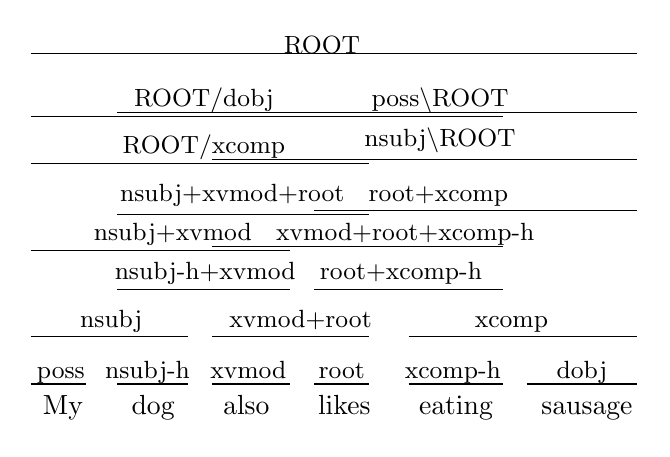
\begin{tikzpicture}
\node at (4,0) {My \hskip 5mm dog \hskip 5mm  also \hskip 5mm  likes \hskip 5mm  eating \hskip 5mm  sausage};
\draw (0.1, 0.3) -- (0.8,0.3);	%my
\draw (1.2, 0.3) -- (2.1,0.3);	%dog
\draw (2.4, 0.3) -- (3.4,0.3);	%also
\draw (3.7, 0.3) -- (4.4,0.3);	%likes
\draw (4.9,0.3) -- (6.1,0.3);	%eating
\draw (6.4,0.3) -- (7.8,0.3);	%sausage
\draw (3.8,0.45) node [font=\small] {poss \hskip 1.5mm nsubj-h \hskip 1.5mm xvmod \hskip 3mm root \hskip 4mm xcomp-h \hskip 6mm dobj};

\draw (0.1, 0.9) -- (2.1, 0.9);	%my dog
\draw (2.4,0.9) -- (4.4,0.9);	%also likes
\draw (4.9,0.9) -- (7.8,0.9);	%eating sausage
\draw (1.2,1.5) -- (3.4, 1.5);	%dog also
\draw (3.7,1.5) -- (6.1, 1.5);	%likes eating
\draw (3.7,1.1) node [font=\small] {nsubj \hskip 10mm xvmod+root \hskip 12mm xcomp};
\draw (3.5,1.7) node [font=\small] {nsubj-h+xvmod \hskip 2mm root+xcomp-h};

\draw (0.1,2) -- (3.4, 2); %my dog also
\draw (3.7,2.5) -- (7.8,2.5); %likes eating sausage
\draw (1.2, 2.45) -- (4.4, 2.45) ;	%dog also likes
\draw (2.4,2.05) -- (6.1,2.05); %also likes eating
\draw (3.7, 2.2) node [font=\small] {nsubj+xvmod \hskip 2mm xvmod+root+xcomp-h};
\draw (3.7, 2.7) node [font=\small] {nsubj+xvmod+root \hskip 2mm root+xcomp};

\draw (0.1,3.1) -- (4.4,3.1);
\draw (2.4,3.15) -- (7.8, 3.15);
\draw (2.3,3.3) node [font=\small] {ROOT/xcomp};
\draw (5.3,3.4) node [font=\small] {nsubj\textbackslash ROOT};

\draw (0.1,3.7) -- (6.1,3.7);
\draw (1.2,3.75) -- (7.8, 3.75);
\draw (2.3,3.9) node [font=\small] {ROOT/dobj};
\draw (5.3,3.9) node [font=\small] {poss\textbackslash ROOT};

\draw (0.1,4.5) -- (7.8, 4.5);
\draw (3.8, 4.6) node [font=\small] {ROOT};

\end{tikzpicture}
\caption{SAMT labels}\label{fig:SAMT}
\end{figure}

In this sentence, only the span covering words 1 to 4 does not have a label. A test on the first 10,000 sentences of our datasets showed that on average less than 60\% of the translation admissible spans in the 4 automatically aligned datasets were assigned a label different from FAIL (see Table \ref{tab:SAMT}).

\begin{table}
\begin{tabular}{|l|l|l|l|}
\hline
\textbf{Language pair} & \textbf{Spans total} & \textbf{Spans labelled SAMT} & \textbf{\% Labelled}\\
\hline \hline
English-Dutch & 1078307 & 598583 & 0.56\\
\hline
English-French & 1260720 & 644710 & 0.51\\
\hline
English-German & 930273 & 540968 & 0.58\\
\hline
English-Chinese & 609401 & 375765 & 0.62\\
\hline
\end{tabular}
\caption{Success rate of SAMT labels}\label{tab:SAMT}
\end{table}

\subsubsection{Extended Labelling}

For the purpose of detecting similarities, the percentage of labelled spans should be as high as possible. We propose the following method for labelling \textit{all} spans, based on dependency labels, in which we use the basic operations $/$, $+$ and $\backslash$ as before. Algorithm \ref{alg:label_all} describes how to label all spans.

\begin{algorithm}
\caption{Label all spans}\label{alg:label_all}
\begin{algorithmic}
\STATE Return a label for span $(i,j)$, given a set of basic labels $\mathcal{L}$
\IF{$\exists L\in\mathcal{L}$ for $(i,j)$}
		\RETURN $L$
\ELSE
	\STATE n = 2
	\WHILE{1}
		\IF{$\exists A_1,\ldots, A_n \in\mathcal{L}$ s.t. $A_1+\cdots+A_n$ is a label for $(i,j)$}
			\RETURN $A_1+\cdots+A_n$
		\ELSIF{$\exists A_1,\ldots, A_n \in\mathcal{L}$ s.t.$A_1/A_2+\cdots+A_n$ is a label for $(i,j)$}
			\RETURN $A_1/A_2+\cdots+A_n$
		\ELSIF{$\exists A_1,\ldots, A_n \in\mathcal{L}$ s.t. $A_1+\cdots+A_{n-1}\backslash A_n$ is a label for $(i,j)$}
			\RETURN $A_1+\cdots A_{n-1}\backslash A_n$
		\ELSIF{$\exists A_1,\ldots, A_n \in\mathcal{L}$ s.t. $A_1+\cdots+A_{k-1}\backslash A_k/A_{k+1}+\cdots+A_n$ is a label for $(i,j)$}
		\RETURN $A_1+\cdots+A_{k-1}\backslash A_k/A_{k+1}+\cdots+A_n$
		\ELSE
			\STATE n $\leftarrow$ n+1
		\ENDIF
	\ENDWHILE
\ENDIF
\end{algorithmic}
\end{algorithm}

For the previously unlabelled span covering word 1 to 5, Algorithm \ref{alg:label_all} finds the label `$poss\backslash ROOT/dobj$'.

\subsection{Learning the grammar}

With all spans labelled, we can design a learning algorithm that learns a PCFG predicting the HATforest.\footnote{For computational reasons, we have chosen for a PCFG, but similar algorithms can of course be devised to train, e.g., a grammar incorporating larger fragments.} However, to learn a grammar from the data, a probability distribution over the trees in the corpus is required. If such a distribution was known, relative frequency estimation could be used to determine the PCFG that generated it. On the other hand, if the grammar was known, the probability distribution over the HATs would be easy to compute. This chicken and egg problem should seem familiar to statistical modellers. Fortunately, there is an algorithm that addresses the situation of incomplete data: the expectation maximization (EM) algorithm\footnote{This same algorithm was used in the IBM models to determine word-alignments of parallel corpora.} \citep{dempster1977maximum}, that iteratively learns a model from the data, and estimates the data from the model. The EM algorithm is known to converge to a (local) optimum.

\subsubsection{EM for HATs}

In the case of learning a grammar from a set of HATs whose probability distribution is known, the EM algorithm has the following steps:\begin{enumerate}
\item Initialize the model. Typically, this could be done by either distributing the probability mass uniformly over all rules (with the same left-hand side), or by distributing the probability mass uniformly over all HATs (for one sentence), and read of the model by relative frequency estimation
\item For every sentence, compute the probability distribution over its HATs, normalise such that the HAT probabilities sum up to 1 (expectation step).
\item Use relative frequency estimation to learn a new PCFG from the data (maximization step).
\item Iterate 2 and 3 until convergence.
\end{enumerate}

\subsubsection{Computation}

Of course, naively following the protocol described in the previous subsection would not be computationally feasible. As the HATs are implicitly represented as CFGs, explicitly computing the probability of all HATs would require unpacking the entire HATforest, which grows exponentially with the length of the sentence. This would not only be time and space consuming, but would also require a lot of redundant computing, as the probability of subtrees that occur in multiple HATs need to be recomputed many times.

In this subsection, we propose an algorithm for computing the updates for one EM iteration without unpacking the HATforest, that focusses on reusing previously computed values and using only a limited amount of memory at a certain time. The algorithm describes how to compute the updates (i.e., the relative frequency counts) of the HAT grammar for one sentence, given the grammar that was computed in the previous EM iteration. It is assumed that the HAT grammars for all sentences are stored, and can be requested. The following abbreviations are used:\begin{enumerate}
\item $P(A)$ is the sum of the probabilities of all subtrees of HATs headed by the node labelled $A$.
\item $P(A_{x_1\cdots x_n})$ is the sum of the probabilities of all subtrees of HATs headed by $A (x_1 \cdots x_n)$ 
\end{enumerate}

This probability function, that is used in computing the updates, can be precomputed in a top-down fashion, by calling the function described in Algorithm \ref{alg:prob} on the topnode of the HATforest.

\begin{algorithm}
\caption{$prob(\Pp, \Hg,\G,X,(y_1,\cdots,y_n) = None$)}\label{alg:prob}
\begin{algorithmic}
\STATE \textbf{Input:} a dictionary with already computed probabilities $\Pp$, a HATgrammar $\Hg$, a global PCFG $\G$, a node $X$ in $\Hg$, and optionally a set of children in $(y_1\cdots y_n)$ such that $X\rightarrow y_1~\cdots y_n$ is a rule in $\Hg$
\STATE
\IF{$X \in \Pp$}
	\RETURN $\Pp(X)$
	\STATE
\ELSIF{$\neg\exists X\rightarrow C_1~\cdots ~C_N \in\Hg$}
	\RETURN $\Pp(X)=1$
	\STATE
\ELSIF{$(y_1\cdots y_n)!=$None}
	\RETURN $\Pp(X_{y_1\cdots y_n}) = \G(X\rightarrow y_1~\cdots y_n)\cdot\prod_{n}prob(\Hg,\G,y_n)$
	\STATE
\ELSE
	\RETURN $\sum_{X\rightarrow y_1~\cdots ~y_n \in\Hg} \Pp(X_{y_1~\cdots y_n})$
	\STATE
\ENDIF
\end{algorithmic}
\end{algorithm}

To compute the updated count of a rule, one must know in which HATs the rule occurred, and what the probability of these HATs was. This information will be obtained by going through the HAT grammar in a top-down fashion, and computing the (normalised) probability mass of all HATs the rule occurred in, using the probability mass of all subtrees headed by its parent, and the relative probability mass of all subtrees headed by the expansion with respect to other expansions. 
The update process starts by calling the update function described in Algorithm \ref{alg:update} on the topnode of the HATforest. New function calls will be made while computing the probabilities of the productions with this topnode as left-hand side. Counts for productions can be updated multiple times for each rule. Note that it is assued that the algorithm does not return anything, but merely updates a global dictionary with counts for rules. Furthermore, it is assumed that the nodes of the HATs are uniquely defined by their label. The overall complexity of computing the update for a sentence is polynomial in its length (compute precise).

\begin{algorithm}[!ht]
\caption{$update(N,\Hg,\G,\Pp,\C,p_{total})$}\label{alg:update}
\begin{algorithmic}
\STATE \textbf{Input:} a HAtforest $\Hg$, a global grammar $\G$, a function $\Pp$, the current counts $\C$, a node $N$ and a number $p_{total}$ describing the probability mass that is assigned to the parent $N$
\STATE
\IF{$\neg \exists N\rightarrow X_1~\cdots X_n\in\Hg$}
	\RETURN
\ENDIF
\FOR{$R = N\rightarrow X_1~\cdots X_n\in\Hg$}
	\STATE $C_{new} = p_{total}\cdot\frac{\Pp(N_{X_1\cdots X_n})}{\Pp(N)}$
	\STATE $\C(N\rightarrow X_1\cdots X_n) \leftarrow \C(N\rightarrow X_1\cdots X_n) + C_{new}  $
	\FOR{$X\in \{X_1,\cdots X_n\}$}
		\STATE $update(X,\Hg,\G,\Pp,\C,C_{new}))$
	\ENDFOR
\ENDFOR
\end{algorithmic}
\end{algorithm}

The above mentioned algorithms can be used to train a grammar that assigns probabilities to the maximally recursive structures in the corpus.

\section{In conclusion}

In this thesis, we have studied compositional translation on an empirical level. We have elaborately discussed several aspects of compositional translation, and presented a careful analysis of the usefulness of dependency parses for constructing a compositional translation system. Although a conclusive answer to the most general question - can dependency parses be used to construct a bilingual compositional grammar - was not yet found, we believe a useful foundation was created to answer this question. This thesis provides insights to the empirical investigation of compositionality in general, a thorough investigation of dependency parses in the light of compositional translation, a worked out proposal to extend this research, and package of comprehensible and well documented classes that can be used to conduct this, and further research in the same category. 

Although we believe that in the nearby future, developing systems that can automatically produce high quality translations from one natural language will remain a difficult challenge for both the academic and business world, we hope that this work can eventually contribute to being able to proceed to decode.




%\bibliography{thesisDH}
%\end{document}